The system has been modelled using controllers for most of the components. To avoid duplication of code, the two airlocks have the same controller code, and the two controllers are distinguished by means of airlock IDs.

Likewise, both output stacks' interactions, the input stacks' interactions, and the two outer robot controller interactions have the same code in each case, and are differentiated using output stack IDs, input stack IDs, and robot IDs, respectively.

Each controller has a set of states defined by variables as required to determine the uniqueness of the states. State information is exchanged between controllers by means of communication actions described in chapter~{\ref{chap:interact}, and state transitions are made accordingly, based on information received from other controllers.
\\
Here, we describe in brief how the controllers are modelled, and their respective communication actions (the exact code can be found in the Appendix):
\begin{enumerate}
    \item Outer Robot Controller: Makes the robot check the corresponding input stack's state and pick up a wafer if the stack is not empty. Communicates with the airlock controller to determine when to make the robot pick up or drop a wafer. If the robot has a wafer, the controller makes it check the output stack to drop a wafer if the stack is not full. 
    \item Inner Robot Controller: Communicates with the airlock to determine when to pick up or drop a wafer. Makes the robot check the lamp sensor to determine if the wafer is projected or not. Has non-determinism in its logic to make the robot visit one of the airlocks without any priority in case both happen to have unprojected wafers at the same time.
    \item Airlock Controller: Communicates with the inner robot and the airlock's corresponding outer robot to determine which door to open/close. Ensures that the airlock never has both doors open at the same time.
\end{enumerate}

Since there are lots of \textit{IDs} involved, maps have been used to \textit{match} the various IDs across controllers (for instance, when referring to interactions between robot 1 and airlock 1, the IDs will always be matched as $R1 \rightarrow A1$ or $A1 \rightarrow R1$.)
\\\\
Moreover, as stated previously, interactions with the stacks and the lamp are treated as external interactions, and explicit stack and lamp controllers aren't created. We could model controllers for those components as well, but for the sake of keeping the system simple and operational with the existing controllers, we have treated the stacks and lamp as mere passive elements with which the existing controllers interact.

The \texttt{mcrl22lps} command is used to generate the lps for the mclr2 code, and is translated to an lts using the \texttt{lps2lts} command. Given the number of parallel components, it is difficult to get a good understanding of the system based on its LTS, and hence the \texttt{ltsview} command is used to visualize the system and its states.

The following figure is the visual representation of the system:

\begin{figure}[h]
\centering
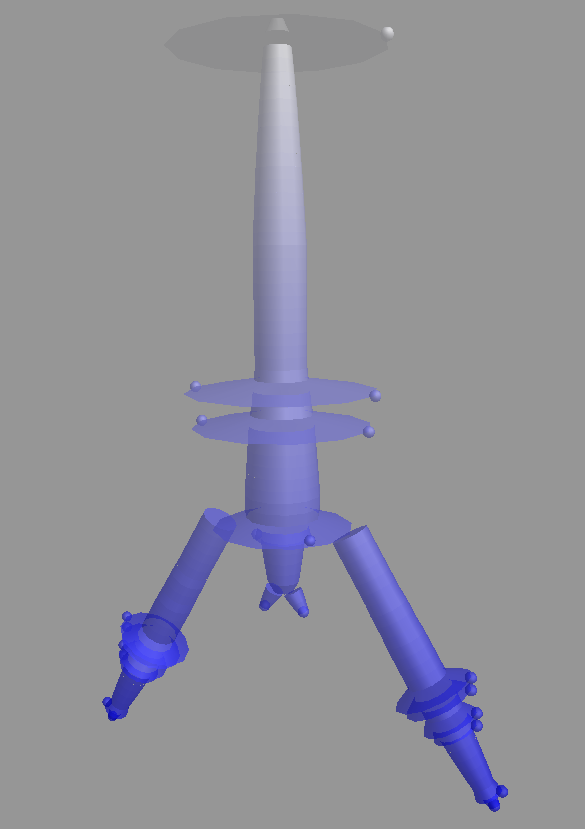
\includegraphics[width=90mm]{img/ltsview.PNG}
\caption{LTS visualization\label{fig:ltsview}}
\end{figure}